%%%%%%%%%%%%%%%%%%%%%%%%%%%%%%%%%%%%%%%%%
% Short Sectioned Assignment
% LaTeX Template
% Version 1.0 (5/5/12)
%
% This template has been downloaded from:
% http://www.LaTeXTemplates.com
%
% Original author:
% Frits Wenneker (http://www.howtotex.com)
%
% License:
% CC BY-NC-SA 3.0 (http://creativecommons.org/licenses/by-nc-sa/3.0/)
%
%%%%%%%%%%%%%%%%%%%%%%%%%%%%%%%%%%%%%%%%%

%----------------------------------------------------------------------------------------
%	PACKAGES AND OTHER DOCUMENT CONFIGURATIONS
%----------------------------------------------------------------------------------------

\documentclass[paper=a4, fontsize=11pt]{scrartcl} % A4 paper and 11pt font size
\usepackage[margin=0.5in]{geometry}
\renewcommand{\thesection}{\Roman{section}}
\usepackage{enumerate}% http://ctan.org/pkg/enumerate
\usepackage[T1]{fontenc} % Use 8-bit encoding that has 256 glyphs
\usepackage{fourier} % Use the Adobe Utopia font for the document - comment this line to return to the LaTeX default
\usepackage[english]{babel} % English language/hyphenation
\usepackage{amsmath,amsfonts,amsthm} % Math packages

\usepackage{lipsum} % Used for inserting dummy 'Lorem ipsum' text into the template

\usepackage{sectsty} % Allows customizing section commands
\usepackage{newlfont} % \Join
\usepackage[absolute,overlay]{textpos}
\usepackage{graphicx}

\allsectionsfont{\centering \normalfont\scshape} % Make all sections centered, the default font and small caps

\usepackage{fancyhdr} % Custom headers and footers
\pagestyle{fancyplain} % Makes all pages in the document conform to the custom headers and footers
\fancyhead{} % No page header - if you want one, create it in the same way as the footers below
\fancyfoot[L]{} % Empty left footer
\fancyfoot[C]{} % Empty center footer
\fancyfoot[R]{\thepage} % Page numbering for right footer
\renewcommand{\headrulewidth}{0pt} % Remove header underlines
\renewcommand{\footrulewidth}{0pt} % Remove footer underlines
\setlength{\headheight}{13.6pt} % Customize the height of the header

\numberwithin{equation}{section} % Number equations within sections (i.e. 1.1, 1.2, 2.1, 2.2 instead of 1, 2, 3, 4)
\numberwithin{figure}{section} % Number figures within sections (i.e. 1.1, 1.2, 2.1, 2.2 instead of 1, 2, 3, 4)
\numberwithin{table}{section} % Number tables within sections (i.e. 1.1, 1.2, 2.1, 2.2 instead of 1, 2, 3, 4)

\setlength\parindent{10pt} % Removes all indentation from paragraphs - comment this line for an assignment with lots of text
\setlength{\parskip}{\baselineskip}%

%----------------------------------------------------------------------------------------
%	TITLE SECTION
%----------------------------------------------------------------------------------------

\newcommand{\horrule}[1]{\rule{\linewidth}{#1}} % Create horizontal rule command with 1 argument of height

\title{	
\normalfont \normalsize \textsc{CS 143, Winter 2015}
\horrule{0.5pt} \\[0.4cm] % Thin top horizontal rule
\huge Lab 3 Write-Up \\ % The assignment title
\horrule{2pt} \\[0.5cm] % Thick bottom horizontal rule
}

\author{Jordi Burbano (204 076 325), Keisuke Daimon (604 547 017)} % Your name

\date{\normalsize 13 March 2015} % Today's date or a custom date

\begin{document}

\maketitle % Print the title

\section{Life of a Query in the SimpleDB System}

%Before executing the query by calling query.execute(), simpledb.Parser.processNextStatement() calls simpledb.Parser.handleQueryStatement().

simpledb.Parser.handleQueryStatement() generates the logical plan lp using parseQueryLogicalPlan. First, the parser walks through the tables in the FROM clause, adding a Scan node to lp for each one. Next, it parses the WHERE clause, creating Filter and Join nodes as needed. It then looks for GROUP BY fields. After that, the parser walks the SELECT list, picks out aggregates, and checks for query validity. Finally, for a ORDER BY clause, it adds an ORDER BY expression to lp in the specified order on the specified field.

handleQueryStatement() then creates a physical plan for the query via a call to lp.physicalPlan().%, which has the following arguments: TransactionId tid, representing the transaction the physical plan will run as a part of; Map<String,TableStats> baseTableStats, which provides a TableStats object for each table referenced by the plan; and boolean explain, which indicates whether output visualizing the physical plan should be given. 
 Initially, for each table, a SeqScan is initialized and the filter selectivity is initialized to 1. Then, to handle the WHERE clause, for each LogicalFilterNode, the corresponding filter selectivity is scaled by the selectivity computed from the relevant TableStats object calling estimateSelectivity(), which in turn uses an IntHistogram or a StringHistogram, depending on the field's type, to compute the selectivity.

%Afterwards, JoinOptimizer.orderJoins() is called to produce a Vector<LogicalJoinNode> object joins. Then walk the select list to determine the order to project output fields. Checking if aggregates and order by are used, the appropriate relation project Project is returned. If the physical plan is not null, the query plan tree is then printed to the standard output stream.

%----------------------------------------------------------------------------------------
%	Design Decisions
%----------------------------------------------------------------------------------------

\section{Design Decisions}

%\subsection{Methods for Selectivity Estimation}

Selectivity estimation is implemented in the IntHistogram class, which makes use of an int[][] histogram hist to estimate different types of selectivities. The histogram double array's first dimension is along individual bins while the second dimension records two numbers: the bin's rightmost value and the bin's count. hist[0] corresponds to a special case in that it is used to keep track of the total number of tuples.

%The width of each bin is computed as (Max - Min + 1) / (Total number of buckets). Because the width is a double value but histogram is an int[][] array, the width is rounded when used to compute each bin's rightmost int value. As a result, in the special case that the total number of buckets exceeds the total width, i.e. width < 1, a given int may map to multiple bins, e.g. bin1's rightmost value may be (int) Math.round(2.1)=2 while bin2's rightmost value would be (int) Math.round(2.4)=2. However, the method addValue() eliminates this ambiguity by mapping an int to the first bin encountered. This subtlety would prove to be the underlying reason for a troublesome bug.

%The method estimateSelectivity() simply makes use of the logic provided in the assignment description to compute the selectivity for each operator.


%\subsection{Methods for Join Ordering}

JoinOptimizer.orderJoins() implements the Selinger optimizer. This method makes use of the provided enumerateSubsets() method in considering each subset with size i, as well as the computeCostAndCardOfSubplan to compute each join cost and cardinality.

\section{Example Query Plans}

The following query was executed:

select d.fname, d.lname\\
from Actor a, Casts c, \texttt{Movie\_Director} m, Director d\\
where a.id=c.pid and c.mid=m.mid and m.did=d.id
and a.fname='John' and a.lname='Spicer';

The following query plan was generated:

\begin{figure}[ht!]
\centering
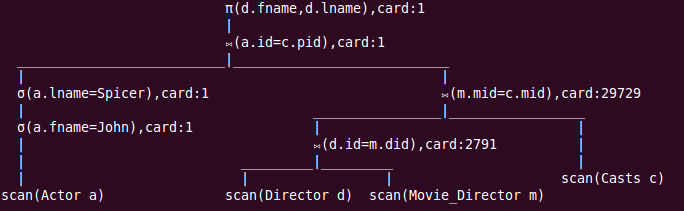
\includegraphics[width=100mm]{queryPlan1.png}
\label{overflow}
\end{figure}

In this counterintuitive plan, the result of applying two selections on the relation Actor is joined last
perhaps because the optimizer erroneously only considers the initial scan cost of Actor, which is the largest
of all relations.

The following query was also executed:

select m.name, g.genre\\
from Movie m, Genre g\\
where m.year=1991 and m.id=g.mid;

The following query plan was then generated:
\begin{figure}[ht!]
\centering
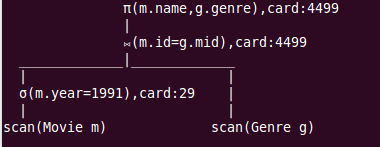
\includegraphics[width=56mm]{queryPlan2.png}
\label{overflow}
\end{figure}

In this plan, as one would expect, the result of applying a selection on the relation Movie
is conditionally joined with Genre g, as opposed to performing the join earlier and the selection later.

%----------------------------------------------------------------------------------------
%	Changes to the API
%----------------------------------------------------------------------------------------

\section{Changes to the API}

We made no changes to the API.



%----------------------------------------------------------------------------------------
%	Missing or Incomplete Elements of Our Code
%----------------------------------------------------------------------------------------

\section{Missing or Incomplete Elements of Our Code}

There are no missing or incomplete elements in our code.



%----------------------------------------------------------------------------------------
%	Logistics
%----------------------------------------------------------------------------------------

\section{Logistics}

We spent approximately 25 man-hours on the project.

%As mentioned in the description of the methods

For selectivity estimation, in the special case of width<1, an int could map to multiple bins even though it would only be placed in one. In this case, the width would have to be scaled by an appropriate factor to account for the other, unused bins, and this is done by replacing width by width<1?1:width in the estimateSelectivity() computations. Previously, the lack of this compensation had resulted in an overestimation by a factor of 3 for computing the selectivity for equality with Min=0, Max=31; this was because width was computed as 32/100=0.32, when the width of a bin, e.g. for the number 4, should actually be 1.

Regarding the time of this assignment's submission, it has been submitted 1 day late; previously, we had 4 slip days available since we had not used any before.


\end{document}